\documentclass{article}
\usepackage[margin=0.75in]{geometry}
\usepackage{tikz}
\usepackage{multicol}
\usepackage{fancyhdr}
\usepackage{xcolor}
\usetikzlibrary{shadows}

\begin{document}

\pagestyle{fancy}
\chead{Mech/Wholetone Layout Cheat Sheet}
\rhead{}
\lhead{}
\cfoot{github.com/flipcoder/midimech}

\section{Intervals}

\begin{multicols}{4}

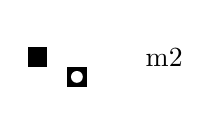
\begin{tikzpicture}[scale=0.25]
  % Draw the grid with transparent borders
  \draw[draw=none, fill=none] (0,0) grid (3,3);
  
  % Fill in and color specific squares
  \fill[black] (2,0) rectangle ++(1,1);
  \fill[white] (2.5,0.5) circle (0.3);
  \fill[black] (0,1) rectangle ++(1,1);
  
  \node[right] at (5.5,1.5) {m2};
\end{tikzpicture}\vspace{.5cm}


\begin{tikzpicture}[scale=0.25]
  % Draw the grid with transparent borders
  \draw[draw=none, fill=none] (0,0) grid (3,3);
  
  % Fill in and color specific squares
  \fill[black] (0,0) rectangle ++(1,1);
  \fill[white] (0.5,0.5) circle (0.3);
  \fill[black] (1,0) rectangle ++(1,1);
  
  \node[right] at (5.5,1.5) {M2};
\end{tikzpicture}\vspace{.5cm}

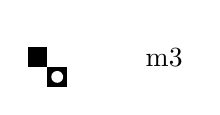
\begin{tikzpicture}[scale=0.25]
  % Draw the grid with transparent borders
  \draw[draw=none, fill=none] (0,0) grid (3,3);
  
  % Fill in and color specific squares
  \fill[black] (1,0) rectangle ++(1,1);
  \fill[white] (1.5,0.5) circle (0.3);
  \fill[black] (0,1) rectangle ++(1,1);
  
  \node[right] at (5.5,1.5) {m3};
\end{tikzpicture}\vspace{.5cm}

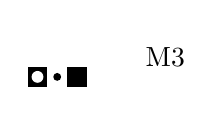
\begin{tikzpicture}[scale=0.25]
  % Draw the grid with transparent borders
  \draw[draw=none, fill=none] (0,0) grid (3,3);
  
  % Fill in and color specific squares
  \fill[black] (0,0) rectangle ++(1,1);
  \fill[white] (0.5,0.5) circle (0.3);
  \fill[black] (1.5,0.5) circle (0.2);
  \fill[black] (2,0) rectangle ++(1,1);
  
  \node[right] at (5.5,1.5) {M3};
\end{tikzpicture}\vspace{.5cm}

\end{multicols}
\begin{multicols}{4}


\begin{tikzpicture}[scale=0.25]
  % Draw the grid with transparent borders
  \draw[draw=none, fill=none] (0,0) grid (3,3);
  
  % Fill in and color specific squares
  \fill[black] (0,0) rectangle ++(1,1);
  \fill[white] (0.5,0.5) circle (0.3);
  \fill[black] (0,1) rectangle ++(1,1);
  
  \node[right] at (5.5,1.5) {P4};
\end{tikzpicture}\vspace{.5cm}

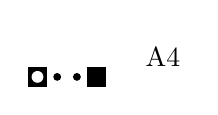
\begin{tikzpicture}[scale=0.25]
  % Draw the grid with transparent borders
  \draw[draw=none, fill=none] (0,0) grid (3,3);
  
  % Fill in and color specific squares
  \fill[black] (0,0) rectangle ++(1,1);
  \fill[white] (0.5,0.5) circle (0.3);
  \fill[black] (1.5,0.5) circle (0.2);
  \fill[black] (2.5,0.5) circle (0.2);
  \fill[black] (3,0) rectangle ++(1,1);
  
  \node[right] at (5.5,1.5) {A4};
\end{tikzpicture}\vspace{.5cm}

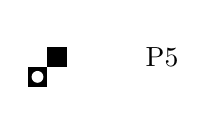
\begin{tikzpicture}[scale=0.25]
  % Draw the grid with transparent borders
  \draw[draw=none, fill=none] (0,0) grid (3,3);
  
  % Fill in and color specific squares
  \fill[black] (0,0) rectangle ++(1,1);
  \fill[white] (0.5,0.5) circle (0.3);
  \fill[black] (1,1) rectangle ++(1,1);
  
  \node[right] at (5.5,1.5) {P5};
\end{tikzpicture}\vspace{.5cm}

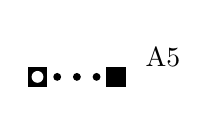
\begin{tikzpicture}[scale=0.25]
  % Draw the grid with transparent borders
  \draw[draw=none, fill=none] (0,0) grid (3,3);
  
  % Fill in and color specific squares
  \fill[black] (0,0) rectangle ++(1,1);
  \fill[white] (0.5,0.5) circle (0.3);
  \fill[black] (1.5,0.5) circle (0.2);
  \fill[black] (2.5,0.5) circle (0.2);
  \fill[black] (3.5,0.5) circle (0.2);
  \fill[black] (4,0) rectangle ++(1,1);
  
  \node[right] at (5.5,1.5) {A5};
\end{tikzpicture}\vspace{.5cm}

\end{multicols}
\begin{multicols}{4}


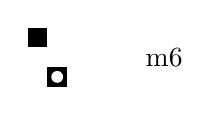
\begin{tikzpicture}[scale=0.25]
  % Draw the grid with transparent borders
  \draw[draw=none, fill=none] (0,0) grid (3,3);
  
  % Fill in and color specific squares
  \fill[black] (1,0) rectangle ++(1,1);
  \fill[white] (1.5,0.5) circle (0.3);
  \fill[black] (0,2) rectangle ++(1,1);
  
  
  \node[right] at (5.5,1.5) {m6};
\end{tikzpicture}\vspace{.5cm}

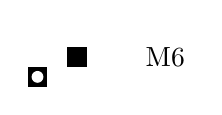
\begin{tikzpicture}[scale=0.25]
  % Draw the grid with transparent borders
  \draw[draw=none, fill=none] (0,0) grid (3,3);
  
  % Fill in and color specific squares
  \fill[black] (0,0) rectangle ++(1,1);
  \fill[white] (0.5,0.5) circle (0.3);
  \fill[black] (2,1) rectangle ++(1,1);
  
  \node[right] at (5.5,1.5) {M6};
\end{tikzpicture}\vspace{.5cm}

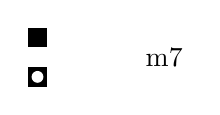
\begin{tikzpicture}[scale=0.25]
  % Draw the grid with transparent borders
  \draw[draw=none, fill=none] (0,0) grid (3,3);
  
  % Fill in and color specific squares
  \fill[black] (0,0) rectangle ++(1,1);
  \fill[white] (0.5,0.5) circle (0.3);
  \fill[black] (0,2) rectangle ++(1,1);
  
  \node[right] at (5.5,1.5) {m7};
\end{tikzpicture}\vspace{.5cm}

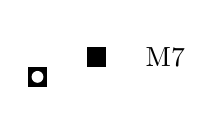
\begin{tikzpicture}[scale=0.25]
  % Draw the grid with transparent borders
  \draw[draw=none, fill=none] (0,0) grid (3,3);
  
  % Fill in and color specific squares
  \fill[black] (0,0) rectangle ++(1,1);
  \fill[white] (0.5,0.5) circle (0.3);
  \fill[black] (3,1) rectangle ++(1,1);
  
  \node[right] at (5.5,1.5) {M7};
\end{tikzpicture}\vspace{.5cm}

\end{multicols}

\section{Chords}

\begin{multicols}{4}

% MAJOR

\begin{tikzpicture}[scale=0.25]
  % Draw the grid with transparent borders
  \draw[draw=none, fill=none] (0,0) grid (3,3);
  
  % Fill in and color specific squares
  \fill[black] (0,0) rectangle ++(1,1);
  \fill[white] (0.5,0.5) circle (0.3);
  \fill[black] (1,1) rectangle ++(1,1);
  \fill[black] (2,0) rectangle ++(1,1);
  
  \node[right] at (5.5,1.5) {major};
\end{tikzpicture}\vspace{.5cm}

% MINOR

\begin{tikzpicture}[scale=0.25]
  % Draw the grid with transparent borders
  \draw[draw=none, fill=none] (0,0) grid (3,3);
  
  % Fill in and color specific squares
  \fill[black] (0,1) rectangle ++(1,1);
  \fill[black] (1,0) rectangle ++(1,1);
  \fill[white] (1.5,0.5) circle (0.3);
  \fill[black] (2,1) rectangle ++(1,1);
  
  \node[right] at (5.5,1.5) {minor};
\end{tikzpicture}\vspace{.5cm}

% SUS2

\begin{tikzpicture}[scale=0.25]
  % Draw the grid with transparent borders
  \draw[draw=none, fill=none] (0,0) grid (3,3);
  
  % Fill in and color specific squares
  \fill[black] (0,0) rectangle ++(1,1);\
  \fill[white] (0.5,0.5) circle (0.3);
  \fill[black] (1,0) rectangle ++(1,1);
  \fill[black] (1,1) rectangle ++(1,1);
  
  \node[right] at (5.5,1.5) {sus2};
\end{tikzpicture}\vspace{.5cm}

% SUS4

\begin{tikzpicture}[scale=0.25]
  % Draw the grid with transparent borders
  \draw[draw=none, fill=none] (0,0) grid (3,3);
  
  % Fill in and color specific squares
  \fill[black] (0,0) rectangle ++(1,1);\
  \fill[white] (0.5,0.5) circle (0.3);
  \fill[black] (0,1) rectangle ++(1,1);
  \fill[black] (1,1) rectangle ++(1,1);
  
  \node[right] at (5.5,1.5) {sus4};
\end{tikzpicture}\vspace{.5cm}

\end{multicols}
\begin{multicols}{4}

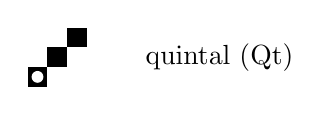
\begin{tikzpicture}[scale=0.25]
  % Draw the grid with transparent borders
  \draw[draw=none, fill=none] (0,0) grid (3,3);
  
  % Fill in and color specific squares
  \fill[black] (0,0) rectangle ++(1,1);\
  \fill[white] (0.5,0.5) circle (0.3);
  \fill[black] (2,2) rectangle ++(1,1);
  \fill[black] (1,1) rectangle ++(1,1);
  
  \node[right] at (5.5,1.5) {quintal (Qt)};
\end{tikzpicture}\vspace{.5cm}


\begin{tikzpicture}[scale=0.25]
  % Draw the grid with transparent borders
  \draw[draw=none, fill=none] (0,0) grid (3,3);
  
  % Fill in and color specific squares
  \fill[black] (0,0) rectangle ++(1,1);\
  \fill[white] (0.5,0.5) circle (0.3);
  \fill[black] (0,1) rectangle ++(1,1);
  \fill[black] (0,2) rectangle ++(1,1);
  
  \node[right] at (5.5,1.5) {quartal (Q)};
\end{tikzpicture}\vspace{.5cm}

% AUGMENTED
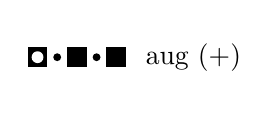
\begin{tikzpicture}[scale=0.25]
  % Draw the grid with transparent borders
  \draw[draw=none, fill=none] (0,0) grid (3,3);
  
  % Fill in and color specific squares
  \fill[black] (0,1) rectangle ++(1,1);\
  \fill[white] (0.5,1.5) circle (0.3);
  \fill[black] (1.5,1.5) circle (0.2);
  \fill[black] (2,1) rectangle ++(1,1);
  \fill[black] (3.5,1.5) circle (0.2);
  \fill[black] (4,1) rectangle ++(1,1);
  
  \node[right] at (5.5,1.5) {aug (+)};
\end{tikzpicture}\vspace{.5cm}

% DIMINISHED
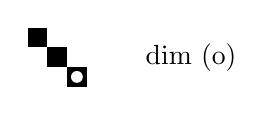
\begin{tikzpicture}[scale=0.25]
  % Draw the grid with transparent borders
  \draw[draw=none, fill=none] (0,0) grid (3,3);
  
  % Fill in and color specific squares
  \fill[black] (0,2) rectangle ++(1,1);\
  \fill[black] (1,1) rectangle ++(1,1);
  \fill[black] (2,0) rectangle ++(1,1);
  \fill[white] (2.5,0.5) circle (0.3);
  
  \node[right] at (5.5,1.5) {dim (o)};
\end{tikzpicture}\vspace{.5cm}

\end{multicols}
\begin{multicols}{4}

% MAJ7
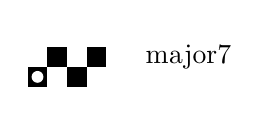
\begin{tikzpicture}[scale=0.25]
  % Draw the grid with transparent borders
  \draw[draw=none, fill=none] (0,0) grid (3,3);
  
  % Fill in and color specific squares
  \fill[black] (0,0) rectangle ++(1,1);
  \fill[white] (0.5,0.5) circle (0.3);
  \fill[black] (1,1) rectangle ++(1,1);
  \fill[black] (2,0) rectangle ++(1,1);
  \fill[black] (3,1) rectangle ++(1,1);
  
  \node[right] at (5.5,1.5) {major7};
\end{tikzpicture}\vspace{.5cm}

% m7
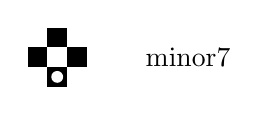
\begin{tikzpicture}[scale=0.25]
  % Draw the grid with transparent borders
  \draw[draw=none, fill=none] (0,0) grid (3,3);
  
  % Fill in and color specific squares
  \fill[black] (0,1) rectangle ++(1,1);
  \fill[black] (1,2) rectangle ++(1,1);
  \fill[black] (2,1) rectangle ++(1,1);
  \fill[black] (1,0) rectangle ++(1,1);
  \fill[white] (1.5,0.5) circle (0.3);
  
  \node[right] at (5.5,1.5) {minor7};
\end{tikzpicture}\vspace{.5cm}

% DOM7
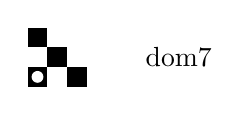
\begin{tikzpicture}[scale=0.25]
  % Draw the grid with transparent borders
  \draw[draw=none, fill=none] (0,0) grid (3,3);
  
  % Fill in and color specific squares
  \fill[black] (0,2) rectangle ++(1,1);
  \fill[black] (0,0) rectangle ++(1,1);
  \fill[white] (0.5,0.5) circle (0.3);
  \fill[black] (1,1) rectangle ++(1,1);
  \fill[black] (2,0) rectangle ++(1,1);
  
  \node[right] at (5.5,1.5) {dom7};
\end{tikzpicture}\vspace{.5cm}

% dim7
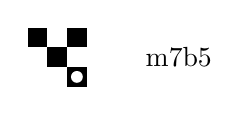
\begin{tikzpicture}[scale=0.25]
  % Draw the grid with transparent borders
  \draw[draw=none, fill=none] (0,0) grid (3,3);
  
  % Fill in and color specific squares
  \fill[black] (0,2) rectangle ++(1,1);
  \fill[black] (1,1) rectangle ++(1,1);
  \fill[black] (2,0) rectangle ++(1,1);
  \fill[white] (2.5,0.5) circle (0.3);
  \fill[black] (2,2) rectangle ++(1,1);
  
  \node[right] at (5.5,1.5) {m7b5};
\end{tikzpicture}\vspace{.5cm}

\end{multicols}
\begin{multicols}{4}

% DIMINISHED 7
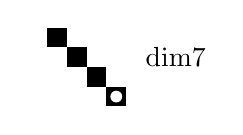
\begin{tikzpicture}[scale=0.25]
  % Draw the grid with transparent borders
  \draw[draw=none, fill=none] (0,0) grid (3,3);
  
  % Fill in and color specific squares
  \fill[black] (4,-1) rectangle ++(1,1);
  \fill[white] (4.5,-0.5) circle (0.3);
  \fill[black] (1,2) rectangle ++(1,1);
  \fill[black] (2,1) rectangle ++(1,1);
  \fill[black] (3,0) rectangle ++(1,1);
  
  \node[right] at (5.5,1.5) {dim7};
\end{tikzpicture}\vspace{.5cm}

% AUGMENTED
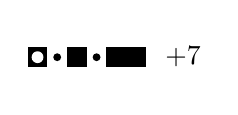
\begin{tikzpicture}[scale=0.25]
  % Draw the grid with transparent borders
  \draw[draw=none, fill=none] (0,0) grid (3,3);
  
  % Fill in and color specific squares
  \fill[black] (0,1) rectangle ++(1,1);\
  \fill[white] (0.5,1.5) circle (0.3);
  \fill[black] (1.5,1.5) circle (0.2);
  \fill[black] (2,1) rectangle ++(1,1);
  \fill[black] (3.5,1.5) circle (0.2);
  \fill[black] (4,1) rectangle ++(1,1);
  \fill[black] (5,1) rectangle ++(1,1);
  
  \node[right] at (6.5,1.5) {+7};
\end{tikzpicture}\vspace{.5cm}

% AUGMENTED
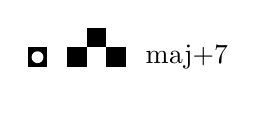
\begin{tikzpicture}[scale=0.25]
  % Draw the grid with transparent borders
  \draw[draw=none, fill=none] (0,0) grid (3,3);
  
  % Fill in and color specific squares
  \fill[black] (0,1) rectangle ++(1,1);\
  \fill[white] (0.5,1.5) circle (0.3);
  \fill[black] (2,1) rectangle ++(1,1);
  \fill[black] (3,2) rectangle ++(1,1);
  \fill[black] (4,1) rectangle ++(1,1);
  
  \node[right] at (5.5,1.5) {maj+7};
\end{tikzpicture}\vspace{.5cm}

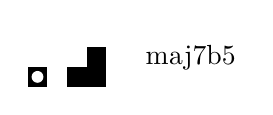
\begin{tikzpicture}[scale=0.25]
  % Draw the grid with transparent borders
  \draw[draw=none, fill=none] (0,0) grid (3,3);
  
  % Fill in and color specific squares
  \fill[black] (0,0) rectangle ++(1,1);
  \fill[white] (0.5,0.5) circle (0.3);
  \fill[black] (3,0) rectangle ++(1,1);
  \fill[black] (2,0) rectangle ++(1,1);
  \fill[black] (3,1) rectangle ++(1,1);
  
  \node[right] at (5.5,1.5) {maj7b5};
\end{tikzpicture}\vspace{.5cm}

\end{multicols}
\begin{multicols}{4}

% MINORMAJOR7
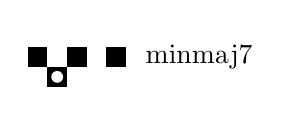
\begin{tikzpicture}[scale=0.25]
  % Draw the grid with transparent borders
  \draw[draw=none, fill=none] (0,0) grid (3,3);
  
  % Fill in and color specific squares
  \fill[black] (0,1) rectangle ++(1,1);
  \fill[black] (1,0) rectangle ++(1,1);
  \fill[white] (1.5,0.5) circle (0.3);
  \fill[black] (2,1) rectangle ++(1,1);
  \fill[black] (4,1) rectangle ++(1,1);
  
  \node[right] at (5.5,1.5) {minmaj7};
\end{tikzpicture}\vspace{.5cm}

% MAJOR6

\begin{tikzpicture}[scale=0.25]
  % Draw the grid with transparent borders
  \draw[draw=none, fill=none] (0,0) grid (3,3);
  
  % Fill in and color specific squares
  \fill[black] (0,0) rectangle ++(1,1);
  \fill[white] (0.5,0.5) circle (0.3);
  \fill[black] (1,1) rectangle ++(1,1);
  \fill[black] (2,0) rectangle ++(1,1);
  \fill[black] (2,1) rectangle ++(1,1);
  
  \node[right] at (5.5,1.5) {maj6};
\end{tikzpicture}\vspace{.5cm}

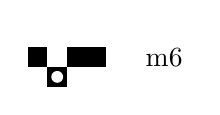
\begin{tikzpicture}[scale=0.25]
  % Draw the grid with transparent borders
  \draw[draw=none, fill=none] (0,0) grid (3,3);
  
  % Fill in and color specific squares
  \fill[black] (1,0) rectangle ++(1,1);
  \fill[white] (1.5,0.5) circle (0.3);
  \fill[black] (0,1) rectangle ++(1,1);
  \fill[black] (2,1) rectangle ++(1,1);
  \fill[black] (3,1) rectangle ++(1,1);
  
  \node[right] at (5.5,1.5) {m6};
\end{tikzpicture}\vspace{.5cm}

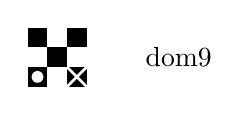
\begin{tikzpicture}[scale=0.25]
  % Draw the grid with transparent borders
  \draw[draw=none, fill=none] (0,0) grid (3,3);

  \fill[black] (0,2) rectangle ++(1,1);
  \fill[black] (0,0) rectangle ++(1,1);
  \fill[white] (0.5,0.5) circle (0.3);
  \fill[black] (1,1) rectangle ++(1,1);
  \fill[black] (2,0) rectangle ++(1,1);
  \fill[black] (2,2) rectangle ++(1,1);
  \draw[line width=1pt, white] (2,0) -- ++(1,1);
  \draw[line width=1pt, white] (2,1) -- ++(1,-1);
  
  \node[right] at (5.5,1.5) {dom9};
\end{tikzpicture}\vspace{.5cm}

\end{multicols}
\section{Inversions}
\begin{multicols}{4}

% MAJOR 1st inv
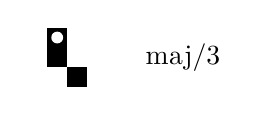
\begin{tikzpicture}[scale=0.25]
  % Draw the grid with transparent borders
  \draw[draw=none, fill=none] (0,0) grid (3,3);
  
  % Fill in and color specific squares
  \fill[black] (1,2) rectangle ++(1,1);
  \fill[white] (1.5,2.5) circle (0.3);
  \fill[black] (1,1) rectangle ++(1,1);
  \fill[black] (2,0) rectangle ++(1,1);

  \node[right] at (5.5,1.5) {maj/3};
\end{tikzpicture}\vspace{.5cm}

% MAJOR 2nd inv

\begin{tikzpicture}[scale=0.25]
  % Draw the grid with transparent borders
  \draw[draw=none, fill=none] (0,0) grid (3,3);
  
  % Fill in and color specific squares
  \fill[black] (0,1) rectangle ++(1,1);
  \fill[white] (0.5,1.5) circle (0.3);
  \fill[black] (0,0) rectangle ++(1,1);
  \fill[black] (2,1) rectangle ++(1,1);
  
  \node[right] at (5.5,1.5) {maj/5};
\end{tikzpicture}\vspace{.5cm}

% MINOR
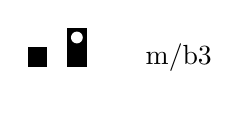
\begin{tikzpicture}[scale=0.25]
  % Draw the grid with transparent borders
  \draw[draw=none, fill=none] (0,0) grid (3,3);
  
  % Fill in and color specific squares
  \fill[black] (0,1) rectangle ++(1,1);
  \fill[black] (2,2) rectangle ++(1,1);
  \fill[white] (2.5,2.5) circle (0.3);
  \fill[black] (2,1) rectangle ++(1,1);
  
  \node[right] at (5.5,1.5) {m/b3};
\end{tikzpicture}\vspace{.5cm}

% MINOR
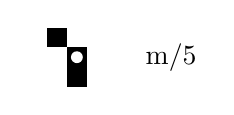
\begin{tikzpicture}[scale=0.25]
  % Draw the grid with transparent borders
  \draw[draw=none, fill=none] (0,0) grid (3,3);
  
  % Fill in and color specific squares
  \fill[black] (1,2) rectangle ++(1,1);
  \fill[black] (2,1) rectangle ++(1,1);
  \fill[white] (2.5,1.5) circle (0.3);
  \fill[black] (2,0) rectangle ++(1,1);
  
  \node[right] at (5.5,1.5) {m/5};
\end{tikzpicture}\vspace{.5cm}

\end{multicols}
\begin{multicols}{4}

% MAJ7 inv1
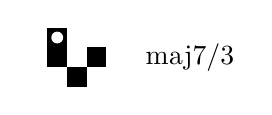
\begin{tikzpicture}[scale=0.25]
  % Draw the grid with transparent borders
  \draw[draw=none, fill=none] (0,0) grid (3,3);
  
  % Fill in and color specific squares
  \fill[black] (1,2) rectangle ++(1,1);
  \fill[white] (1.5,2.5) circle (0.3);
  \fill[black] (1,1) rectangle ++(1,1);
  \fill[black] (2,0) rectangle ++(1,1);
  \fill[black] (3,1) rectangle ++(1,1);
  
  \node[right] at (5.5,1.5) {maj7/3};
\end{tikzpicture}\vspace{.5cm}

% MAJ7 inv2

\begin{tikzpicture}[scale=0.25]
  % Draw the grid with transparent borders
  \draw[draw=none, fill=none] (0,0) grid (3,3);
  
  % Fill in and color specific squares
  \fill[black] (0,1) rectangle ++(1,1);
  \fill[white] (0.5,1.5) circle (0.3);
  \fill[black] (0,0) rectangle ++(1,1);
  \draw[line width=1pt, white] (0,0) -- ++(1,1);
  \draw[line width=1pt, white] (0,1) -- ++(1,-1);
  \fill[black] (2,1) rectangle ++(1,1);
  \fill[black] (2,0) rectangle ++(1,1);
  
  \node[right] at (5.5,1.5) {maj7/5};
\end{tikzpicture}\vspace{.5cm}

% MAJ7 inv2

\begin{tikzpicture}[scale=0.25]
  % Draw the grid with transparent borders
  \draw[draw=none, fill=none] (0,0) grid (3,3);
  
  % Fill in and color specific squares
  \fill[black] (0,1) rectangle ++(1,1);
  \fill[white] (0.5,1.5) circle (0.3);
  \fill[black] (1,2) rectangle ++(1,1);
  \fill[black] (2,1) rectangle ++(1,1);
  \fill[black] (2,0) rectangle ++(1,1);
  
  \node[right] at (5.5,1.5) {maj7/7};
\end{tikzpicture}\vspace{.5cm}

\end{multicols}
\begin{multicols}{4}

% m7/b3
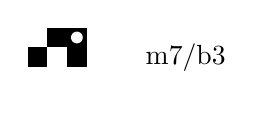
\begin{tikzpicture}[scale=0.25]
  % Draw the grid with transparent borders
  \draw[draw=none, fill=none] (0,0) grid (3,3);
  
  % Fill in and color specific squares
  \fill[black] (0,1) rectangle ++(1,1);
  \fill[black] (1,2) rectangle ++(1,1);
  \fill[black] (2,1) rectangle ++(1,1);
  \fill[black] (2,2) rectangle ++(1,1);
  \fill[white] (2.5,2.5) circle (0.3);
  
  \node[right] at (5.5,1.5) {m7/b3};
\end{tikzpicture}\vspace{.5cm}

% m7/5
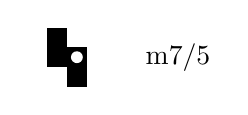
\begin{tikzpicture}[scale=0.25]
  % Draw the grid with transparent borders
  \draw[draw=none, fill=none] (0,0) grid (3,3);
  
  % Fill in and color specific squares
  \fill[black] (1,2) rectangle ++(1,1);
  \fill[black] (1,1) rectangle ++(1,1);
  \fill[black] (2,0) rectangle ++(1,1);
  \fill[black] (2,1) rectangle ++(1,1);
  \fill[white] (2.5,1.5) circle (0.3);
  
  \node[right] at (5.5,1.5) {m7/5};
\end{tikzpicture}\vspace{.5cm}

% m7/b7
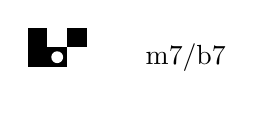
\begin{tikzpicture}[scale=0.25]
  % Draw the grid with transparent borders
  \draw[draw=none, fill=none] (0,0) grid (3,3);
  
  % Fill in and color specific squares
  \fill[black] (0,2) rectangle ++(1,1);
  \fill[black] (0,1) rectangle ++(1,1);
  \fill[black] (2,2) rectangle ++(1,1);
  \fill[black] (1,1) rectangle ++(1,1);
  \fill[white] (1.5,1.5) circle (0.3);
  
  \node[right] at (5.5,1.5) {m7/b7};
\end{tikzpicture}\vspace{.5cm}

\end{multicols}
\begin{multicols}{4}

% 7/3
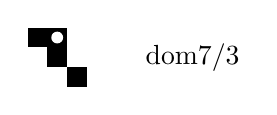
\begin{tikzpicture}[scale=0.25]
  % Draw the grid with transparent borders
  \draw[draw=none, fill=none] (0,0) grid (3,3);
  
  % Fill in and color specific squares
  \fill[black] (0,2) rectangle ++(1,1);
  \fill[black] (1,2) rectangle ++(1,1);
  \fill[white] (1.5,2.5) circle (0.3);
  \fill[black] (1,1) rectangle ++(1,1);
  \fill[black] (2,0) rectangle ++(1,1);
  
  \node[right] at (5.5,1.5) {dom7/3};
\end{tikzpicture}\vspace{.5cm}

% 7/5

\begin{tikzpicture}[scale=0.25]
  % Draw the grid with transparent borders
  \draw[draw=none, fill=none] (0,0) grid (3,3);
  
  % Fill in and color specific squares
  \fill[black] (0,1) rectangle ++(1,1);
  \fill[black] (1,1) rectangle ++(1,1);
  \fill[white] (1.5,1.5) circle (0.3);
  \fill[black] (1,0) rectangle ++(1,1);
  \fill[black] (3,1) rectangle ++(1,1);
  
  \node[right] at (5.5,1.5) {dom7/5};
\end{tikzpicture}\vspace{.5cm}

% 7/b7
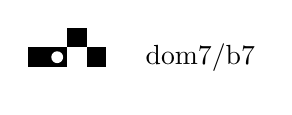
\begin{tikzpicture}[scale=0.25]
  % Draw the grid with transparent borders
  \draw[draw=none, fill=none] (0,0) grid (3,3);
  
  % Fill in and color specific squares
  \fill[black] (0,1) rectangle ++(1,1);
  \fill[black] (1,1) rectangle ++(1,1);
  \fill[white] (1.5,1.5) circle (0.3);
  \fill[black] (2,2) rectangle ++(1,1);
  \fill[black] (3,1) rectangle ++(1,1);
  
  \node[right] at (5.5,1.5) {dom7/b7};
\end{tikzpicture}\vspace{.5cm}


\end{multicols}
\section{Shell Voicings}
\begin{multicols}{4}


\begin{tikzpicture}[scale=0.25]
  % Draw the grid with transparent borders
  \draw[draw=none, fill=none] (0,0) grid (3,3);
  
  \fill[black] (0,0) rectangle ++(1,1);
  \fill[white] (0.5,0.5) circle (0.3);
  \fill[black] (3,2) rectangle ++(1,1);
  \fill[black] (3,1) rectangle ++(1,1);
  
  \node[right] at (5.5,1.5) {maj7};
\end{tikzpicture}\vspace{.5cm}

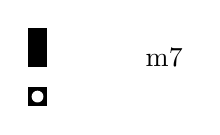
\begin{tikzpicture}[scale=0.25]
  % Draw the grid with transparent borders
  \draw[draw=none, fill=none] (0,0) grid (3,3);
  
  \fill[black] (0,-1) rectangle ++(1,1);
  \fill[white] (0.5,-0.5) circle (0.3);
  \fill[black] (0,2) rectangle ++(1,1);
  \fill[black] (0,1) rectangle ++(1,1);
  
  \node[right] at (5.5,1.5) {m7};
\end{tikzpicture}\vspace{.5cm}

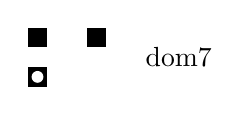
\begin{tikzpicture}[scale=0.25]
  % Draw the grid with transparent borders
  \draw[draw=none, fill=none] (0,0) grid (3,3);
  
  \fill[black] (0,0) rectangle ++(1,1);
  \fill[white] (0.5,0.5) circle (0.3);
  \fill[black] (0,2) rectangle ++(1,1);
  \fill[black] (3,2) rectangle ++(1,1);
  
  \node[right] at (5.5,1.5) {dom7};
\end{tikzpicture}\vspace{.5cm}

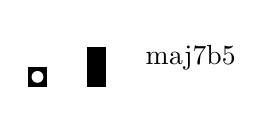
\begin{tikzpicture}[scale=0.25]
  % Draw the grid with transparent borders
  \draw[draw=none, fill=none] (0,0) grid (3,3);
  
  \fill[black] (0,0) rectangle ++(1,1);
  \fill[white] (0.5,0.5) circle (0.3);
  \fill[black] (3,0) rectangle ++(1,1);
  \fill[black] (3,1) rectangle ++(1,1);
  
  \node[right] at (5.5,1.5) {maj7b5};
\end{tikzpicture}\vspace{.5cm}

\end{multicols}
\begin{multicols}{4}

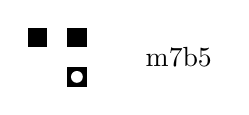
\begin{tikzpicture}[scale=0.25]
  % Draw the grid with transparent borders
  \draw[draw=none, fill=none] (0,0) grid (3,3);
  
  \fill[black] (2,0) rectangle ++(1,1);
  \fill[white] (2.5,0.5) circle (0.3);
  \fill[black] (2,2) rectangle ++(1,1);
  \fill[black] (0,2) rectangle ++(1,1);
  
  \node[right] at (5.5,1.5) {m7b5};
\end{tikzpicture}\vspace{.5cm}

\begin{tikzpicture}[scale=0.25]
  % Draw the grid with transparent borders
  \draw[draw=none, fill=none] (0,0) grid (3,3);
  
  \fill[black] (0,0) rectangle ++(1,1);
  \fill[white] (0.5,0.5) circle (0.3);
  \fill[black] (2,1) rectangle ++(1,1);
  \fill[black] (3,2) rectangle ++(1,1);
  
  \node[right] at (5.5,1.5) {maj6};
\end{tikzpicture}\vspace{.5cm}

\begin{tikzpicture}[scale=0.25]
  % Draw the grid with transparent borders
  \draw[draw=none, fill=none] (0,0) grid (3,3);
  
  % Fill in and color specific squares
  \fill[black] (0,-1) rectangle ++(1,1);
  \fill[white] (0.5,-0.5) circle (0.3);
  \fill[black] (0,2) rectangle ++(1,1);
  \fill[black] (2,0) rectangle ++(1,1);
  
  \node[right] at (5.5,1.5) {m6};
\end{tikzpicture}\vspace{.5cm}

\begin{tikzpicture}[scale=0.25]
  % Draw the grid with transparent borders
  \draw[draw=none, fill=none] (0,0) grid (3,3);
  
  \fill[black] (2,-1) rectangle ++(1,1);
  \fill[white] (2.5,-0.5) circle (0.3);
  \fill[black] (2,2) rectangle ++(1,1);
  \fill[black] (0,2) rectangle ++(1,1);
  
  \node[right] at (5.5,1.5) {minmaj7};
\end{tikzpicture}\vspace{.5cm}

\end{multicols}
\begin{multicols}{4}

\begin{tikzpicture}[scale=0.25]
  % Draw the grid with transparent borders
  \draw[draw=none, fill=none] (0,0) grid (3,3);
  
  \fill[black] (0,0) rectangle ++(1,1);
  \fill[white] (0.5,0.5) circle (0.3);
  \fill[black] (2,2) rectangle ++(1,1);
  \fill[black] (3,2) rectangle ++(1,1);
  \fill[black] (3,1) rectangle ++(1,1);
  
  \node[right] at (5.5,1.5) {maj9};
\end{tikzpicture}\vspace{.5cm}

\begin{tikzpicture}[scale=0.25]
  % Draw the grid with transparent borders
  \draw[draw=none, fill=none] (0,0) grid (3,3);
  
  \fill[black] (0,-1) rectangle ++(1,1);
  \fill[white] (0.5,-0.5) circle (0.3);
  \fill[black] (0,2) rectangle ++(1,1);
  \fill[black] (0,1) rectangle ++(1,1);
  \fill[black] (2,1) rectangle ++(1,1);
  
  \node[right] at (5.5,1.5) {m9};
\end{tikzpicture}\vspace{.5cm}

\begin{tikzpicture}[scale=0.25]
  % Draw the grid with transparent borders
  \draw[draw=none, fill=none] (0,0) grid (3,3);
  
  \fill[black] (0,0) rectangle ++(1,1);
  \fill[white] (0.5,0.5) circle (0.3);
  \fill[black] (0,2) rectangle ++(1,1);
  \fill[black] (3,2) rectangle ++(1,1);
  \fill[black] (2,2) rectangle ++(1,1);
  
  \node[right] at (5.5,1.5) {dom9};
\end{tikzpicture}\vspace{.5cm}

\begin{tikzpicture}[scale=0.25]
  % Draw the grid with transparent borders
  \draw[draw=none, fill=none] (0,0) grid (3,3);
  
  \fill[black] (0,0) rectangle ++(1,1);
  \fill[white] (0.5,0.5) circle (0.3);
  \fill[black] (3,0) rectangle ++(1,1);
  \fill[black] (3,2) rectangle ++(1,1);
  \fill[black] (3,1) rectangle ++(1,1);
  
  \node[right] at (5.5,1.5) {maj\#11};
\end{tikzpicture}\vspace{.5cm}



\end{multicols}

\section{Drop Voicings}
\begin{multicols}{4}

% MAJ7 DROP 2
\begin{tikzpicture}[scale=0.25]
  % Draw the grid with transparent borders
  \draw[draw=none, fill=none] (0,0) grid (3,3);
  
  % Fill in and color specific squares
  \fill[black] (0,1) rectangle ++(1,1);
  \fill[white] (0.5,1.5) circle (0.3);
  \fill[black] (0,0) rectangle ++(1,1);
  \fill[black] (2,1) rectangle ++(1,1);
  \fill[black] (3,2) rectangle ++(1,1);
  
  \node[right] at (5.5,1.5) {maj7(2)};
\end{tikzpicture}\vspace{.5cm}

% MAJ7 DROP 3
\begin{tikzpicture}[scale=0.25]
  % Draw the grid with transparent borders
  \draw[draw=none, fill=none] (0,0) grid (3,3);
  
  % Fill in and color specific squares
  \fill[black] (0,2) rectangle ++(1,1);
  \fill[white] (0.5,2.5) circle (0.3);
  \fill[black] (1,3) rectangle ++(1,1);
  \fill[black] (1,0) rectangle ++(1,1);
  \fill[black] (3,3) rectangle ++(1,1);
  
  \node[right] at (5.5,1.5) {maj7(3)};
\end{tikzpicture}\vspace{.5cm}

% MAJ7 DROP 2+3
\begin{tikzpicture}[scale=0.25]
  % Draw the grid with transparent borders
  \draw[draw=none, fill=none] (0,0) grid (3,3);
  
  % Fill in and color specific squares
  \fill[black] (0,2) rectangle ++(1,1);
  \fill[white] (0.5,2.5) circle (0.3);
  \fill[black] (0,1) rectangle ++(1,1);
  \fill[black] (1,0) rectangle ++(1,1);
  \fill[black] (3,3) rectangle ++(1,1);
  
  \node[right] at (5.5,1.5) {maj7(2,3)};
\end{tikzpicture}\vspace{.5cm}

% MAJ7 DROP 2+4
\begin{tikzpicture}[scale=0.25]
  % Draw the grid with transparent borders
  \draw[draw=none, fill=none] (0,0) grid (3,3);
  
  % Fill in and color specific squares
  \fill[black] (-1,0) rectangle ++(1,1);
  \fill[white] (-0.5,0.5) circle (0.3);
  \fill[black] (0,1) rectangle ++(1,1);
  \fill[black] (2,2) rectangle ++(1,1);
  \fill[black] (3,3) rectangle ++(1,1);
  
  \node[right] at (5.5,1.5) {maj7(2,4)};
\end{tikzpicture}\vspace{.5cm}

\end{multicols}
\begin{multicols}{4}

% m7(2)
\begin{tikzpicture}[scale=0.25]
  % Draw the grid with transparent borders
  \draw[draw=none, fill=none] (0,0) grid (3,3);
  
  % Fill in and color specific squares
  \fill[black] (0,2) rectangle ++(1,1);
  \fill[black] (1,3) rectangle ++(1,1);
  \fill[black] (1,0) rectangle ++(1,1);
  \fill[black] (1,1) rectangle ++(1,1);
  \fill[white] (1.5,1.5) circle (0.3);
  
  \node[right] at (5.5,1.5) {m7(2)};
\end{tikzpicture}\vspace{.5cm}

% m7(3)
\begin{tikzpicture}[scale=0.25]
  % Draw the grid with transparent borders
  \draw[draw=none, fill=none] (0,0) grid (3,3);
  
  % Fill in and color specific squares
  \fill[black] (0,0) rectangle ++(1,1);
  \fill[black] (2,3) rectangle ++(1,1);
  \fill[black] (3,2) rectangle ++(1,1);
  \fill[black] (2,1) rectangle ++(1,1);
  \fill[white] (2.5,1.5) circle (0.3);
  
  \node[right] at (5.5,1.5) {m7(3)};
\end{tikzpicture}\vspace{.5cm}

\begin{tikzpicture}[scale=0.25]
  % Draw the grid with transparent borders
  \draw[draw=none, fill=none] (0,0) grid (3,3);
  
  % Fill in and color specific squares
  \fill[black] (0,0) rectangle ++(1,1);
  \fill[black] (2,3) rectangle ++(1,1);
  \fill[black] (2,0) rectangle ++(1,1);
  \fill[black] (2,1) rectangle ++(1,1);
  \fill[white] (2.5,1.5) circle (0.3);
  
  \node[right] at (5.5,1.5) {m7(2,3)};
\end{tikzpicture}\vspace{.5cm}

\begin{tikzpicture}[scale=0.25]
  % Draw the grid with transparent borders
  \draw[draw=none, fill=none] (0,0) grid (3,3);
  
  % Fill in and color specific squares
  \fill[black] (1,2) rectangle ++(1,1);
  \fill[black] (2,3) rectangle ++(1,1);
  \fill[black] (2,0) rectangle ++(1,1);
  \fill[black] (1,-1) rectangle ++(1,1);
  \fill[white] (1.5,-0.5) circle (0.3);
  
  \node[right] at (5.5,1.5) {m7(2,4)};
\end{tikzpicture}\vspace{.5cm}

\end{multicols}
\begin{multicols}{4}

\begin{tikzpicture}[scale=0.25]
  % Draw the grid with transparent borders
  \draw[draw=none, fill=none] (0,0) grid (3,3);
  
  % Fill in and color specific squares
  \fill[black] (0,2) rectangle ++(1,1);
  \fill[black] (0,0) rectangle ++(1,1);
  \fill[white] (0.5,0.5) circle (0.3);
  \fill[black] (0,-1) rectangle ++(1,1);
  \fill[black] (2,0) rectangle ++(1,1);
  
  \node[right] at (5.5,1.5) {7(2)};
\end{tikzpicture}\vspace{.5cm}

\begin{tikzpicture}[scale=0.25]
  % Draw the grid with transparent borders
  \draw[draw=none, fill=none] (0,0) grid (3,3);
  
  % Fill in and color specific squares
  \fill[black] (0,2) rectangle ++(1,1);
  \fill[black] (0,0) rectangle ++(1,1);
  \fill[white] (0.5,0.5) circle (0.3);
  \fill[black] (1,1) rectangle ++(1,1);
  \fill[black] (1,-2) rectangle ++(1,1);
  
  \node[right] at (5.5,1.5) {7(3)};
\end{tikzpicture}\vspace{.5cm}

\begin{tikzpicture}[scale=0.25]
  % Draw the grid with transparent borders
  \draw[draw=none, fill=none] (0,0) grid (3,3);
  
  % Fill in and color specific squares
  \fill[black] (0,2) rectangle ++(1,1);
  \fill[black] (0,0) rectangle ++(1,1);
  \fill[white] (0.5,0.5) circle (0.3);
  \fill[black] (0,-1) rectangle ++(1,1);
  \fill[black] (1,-2) rectangle ++(1,1);
  
  \node[right] at (5.5,1.5) {7(2,3)};
\end{tikzpicture}\vspace{.5cm}

\begin{tikzpicture}[scale=0.25]
  % Draw the grid with transparent borders
  \draw[draw=none, fill=none] (0,0) grid (3,3);
  
  % Fill in and color specific squares
  \fill[black] (0,2) rectangle ++(1,1);
  \fill[black] (-1,-2) rectangle ++(1,1);
  \fill[white] (-0.5,-1.5) circle (0.3);
  \fill[black] (0,-1) rectangle ++(1,1);
  \fill[black] (2,0) rectangle ++(1,1);
  
  \node[right] at (5.5,1.5) {7(2,4)};
\end{tikzpicture}\vspace{.5cm}

\end{multicols}
\section{Scales}

\begin{multicols}{3}

\begin{tikzpicture}[scale=0.4]
  % Draw the grid with transparent borders
  \draw[draw=none, fill=none] (0,0) grid (3,3);
  
  % Fill in and color specific squares
  \draw (0,0) rectangle ++(1,1);
  \node at (0.5,0.5) {1};
  \draw (1,0) rectangle ++(1,1);
  \node at (1.5,0.5) {2};
  \draw (2,0) rectangle ++(1,1);
  \node at (2.5,0.5) {3};
  \draw (0,1) rectangle ++(1,1);
  \node at (0.5,1.5) {4};
  \draw (1,1) rectangle ++(1,1);
  \node at (1.5,1.5) {5};
  \draw (2,1) rectangle ++(1,1);
  \node at (2.5,1.5) {6};
  \draw (3,1) rectangle ++(1,1);
  \node at (3.5,1.5) {7};
  
  \node[right] at (5.5,1.5) {\textbf{Major}};
\end{tikzpicture}\vspace{.5cm}

\begin{tikzpicture}[scale=0.4]
  % Draw the grid with transparent borders
  \draw[draw=none, fill=none] (0,0) grid (3,3);
  
  % Fill in and color specific squares
  \draw (2,0) rectangle ++(1,1);
  \node at (2.5,0.5) {1};
  \draw (3,0) rectangle ++(1,1);
  \node at (3.5,0.5) {2};
  \draw (1,1) rectangle ++(1,1);
  \node at (1.5,1.5) {3};
  \draw (2,1) rectangle ++(1,1);
  \node at (2.5,1.5) {4};
  \draw (3,1) rectangle ++(1,1);
  \node at (3.5,1.5) {5};
  \draw (1,2) rectangle ++(1,1);
  \node at (1.5,2.5) {6};
  \draw (2,2) rectangle ++(1,1);
  \node at (2.5,2.5) {7};
  
  \node[right] at (5.5,1.5) {\textbf{Minor}};
\end{tikzpicture}\vspace{.5cm}


\begin{tikzpicture}[scale=0.4]
  % Draw the grid with transparent borders
  \draw[draw=none, fill=none] (0,0) grid (3,3);
  
  % Fill in and color specific squares
  \draw (0,0) rectangle ++(1,1);
  \node at (0.5,0.5) {1};
  \draw (1,0) rectangle ++(1,1);
  \node at (1.5,0.5) {2};
  \draw (2,0) rectangle ++(1,1);
  \node at (2.5,0.5) {3};
  \draw (1,1) rectangle ++(1,1);
  \node at (1.5,1.5) {4};
  \draw (2,1) rectangle ++(1,1);
  \node at (2.5,1.5) {5};
  
  \node[right] at (5.5,1.5) {\textbf{Pentatonic}};
\end{tikzpicture}\vspace{.5cm}

\end{multicols}
\begin{multicols}{3}

\begin{tikzpicture}[scale=0.4]
  % Draw the grid with transparent borders
  \draw[draw=none, fill=none] (0,0) grid (3,3);
  
  % Fill in and color specific squares
  \draw (0,0) rectangle ++(1,1);
  \node at (0.5,0.5) {1};
  \draw (1,0) rectangle ++(1,1);
  \node at (1.5,0.5) {2};
  \draw (-1,1) rectangle ++(1,1);
  \node at (-0.5,1.5) {3};
  \draw (0,1) rectangle ++(1,1);
  \node at (0.5,1.5) {4};
  \draw (1,1) rectangle ++(1,1);
  \node at (1.5,1.5) {5};
  \draw (2,1) rectangle ++(1,1);
  \node at (2.5,1.5) {6};
  \draw (3,1) rectangle ++(1,1);
  \node at (3.5,1.5) {7};
  
  \node[right] at (4.5,1.5) {\textbf{Melodic Minor}};
\end{tikzpicture}\vspace{.5cm}

\begin{tikzpicture}[scale=0.4]
  % Draw the grid with transparent borders
  \draw[draw=none, fill=none] (0,0) grid (3,3);
  
  % Fill in and color specific squares
  \draw (0,0) rectangle ++(1,1);
  \node at (0.5,0.5) {1};
  \draw (1,0) rectangle ++(1,1);
  \node at (1.5,0.5) {2};
  \draw (-1,1) rectangle ++(1,1);
  \node at (-0.5,1.5) {3};
  \draw (2,0) rectangle ++(1,1);
  \node at (2.5,0.5) {4};
  \draw (1,1) rectangle ++(1,1);
  \node at (1.5,1.5) {5};
  \draw (2,1) rectangle ++(1,1);
  \node at (2.5,1.5) {6};
  
  \node[right] at (4.5,1.5) {\textbf{Major Blues}};
\end{tikzpicture}\vspace{.5cm}


\begin{tikzpicture}[scale=0.4]
  % Draw the grid with transparent borders
  \draw[draw=none, fill=none] (0,0) grid (3,3);
  
  % Fill in and color specific squares
  \draw (2,0) rectangle ++(1,1);
  \node at (2.5,0.5) {1};
  \draw (1,1) rectangle ++(1,1);
  \node at (1.5,1.5) {2};
  \draw (2,1) rectangle ++(1,1);
  \node at (2.5,1.5) {3};
  \draw (0,2) rectangle ++(1,1);
  \node at (0.5,2.5) {4};
  \draw (3,1) rectangle ++(1,1);
  \node at (3.5,1.5) {5};
  \draw (2,2) rectangle ++(1,1);
  \node at (2.5,2.5) {6};
  
  \node[right] at (5.5,1.5) {\textbf{Minor Blues}};
\end{tikzpicture}\vspace{.5cm}

\end{multicols}
\begin{multicols}{3}

\begin{tikzpicture}[scale=0.4]
  % Draw the grid with transparent borders
  \draw[draw=none, fill=none] (0,0) grid (3,3);
  
  % Fill in and color specific squares
  \draw (1,0) rectangle ++(1,1);
  \node at (1.5,0.5) {1};
  \draw (2,0) rectangle ++(1,1);
  \node at (2.5,0.5) {2};
  \draw (0,1) rectangle ++(1,1);
  \node at (0.5,1.5) {3};
  \draw (1,1) rectangle ++(1,1);
  \node at (1.5,1.5) {4};
  \draw (2,1) rectangle ++(1,1);
  \node at (2.5,1.5) {5};
  \draw (0,2) rectangle ++(1,1);
  \node at (0.5,2.5) {6};
  \draw (4,1) rectangle ++(1,1);
  \node at (4.5,1.5) {7};
  
  \node[right] at (5.5,1.5) {\textbf{Harmonic Minor}};
\end{tikzpicture}\vspace{.5cm}

\begin{tikzpicture}[scale=0.4]
  % Draw the grid with transparent borders
  \draw[draw=none, fill=none] (0,0) grid (3,3);
  
  % Fill in and color specific squares
  \draw (1,0) rectangle ++(1,1);
  \node at (1.5,0.5) {1};
  \draw (2,0) rectangle ++(1,1);
  \node at (2.5,0.5) {2};
  \draw (3,0) rectangle ++(1,1);
  \node at (3.5,0.5) {3};
  \draw (1,1) rectangle ++(1,1);
  \node at (1.5,1.5) {4};
  \draw (2,1) rectangle ++(1,1);
  \node at (2.5,1.5) {5};
  \draw (0,2) rectangle ++(1,1);
  \node at (0.5,2.5) {6};
  \draw (4,1) rectangle ++(1,1);
  \node at (4.5,1.5) {7};
  
  \node[right] at (5.5,1.5) {\textbf{Harmonic Major}};
\end{tikzpicture}\vspace{.5cm}

\begin{tikzpicture}[scale=0.4]
  % Draw the grid with transparent borders
  \draw[draw=none, fill=none] (0,0) grid (3,3);
  
  % Fill in and color specific squares
  
  \node[right] at (5.5,1.5) {\textbf{}};
\end{tikzpicture}\vspace{.5cm}

\end{multicols}

\end{document}

